\section{KI-Client}
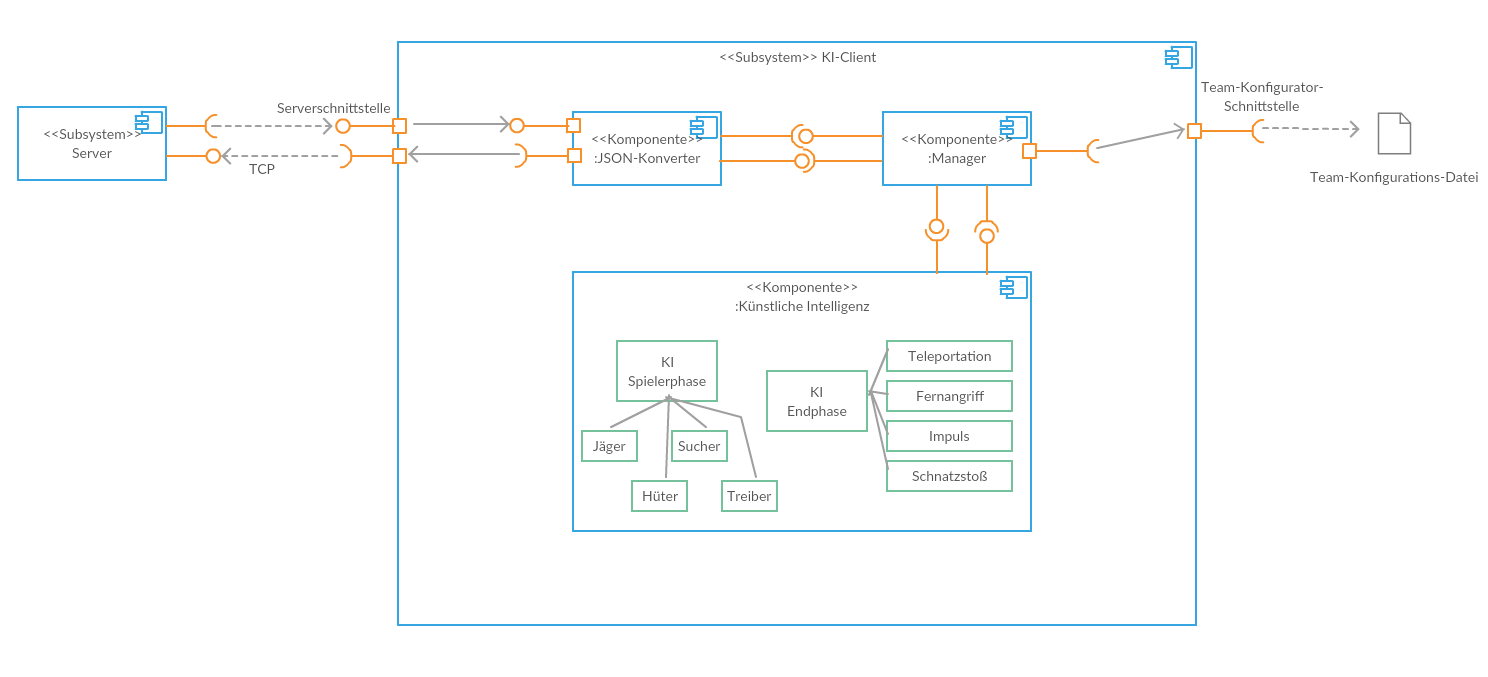
\includegraphics[width=15cm]{images/KI_Client_Komponenten.png}

\begin{description}
	\item[KI-Client:] 
	Das Subsystem KI-Client ist eine Kommandozeilenanwendung, die sich wie ein Nutzer-Client mit einem Server verbindet, einer Partie beitritt und, gesteuert von einer KI, einen menschlichen Spieler simuliert. 
	\\
	\item[Manager:]
	Diese Komponente verwaltet die Daten des KI-Client, insbesondere die aktuelle Spielsituation und verarbeitet die Anwendungsparameter.\\ Der Manager empfängt vom JSON-Konverter die aktuelle Spielsituation und aktualisiert seine gespeicherten Daten entsprechend. Er übergibt seine Daten an die KI, damit diese Entscheidungen über die durchzuführenden Aktionen treffen kann. Anschließend empfängt er die Entscheidungen der KI und aktualisiert die gespeicherte Spielsituation entsprechend, bevor er sie dem JSON-Konverter übergibt.\\
	Außerdem verwaltet der Manager die verwendete Team-Konfiguration. Dabei ist er dafür zuständig, die Konfigurations-Datei im angegebenen Pfad zu öffnen. Die eingelesene Daten übergibt er dann dem JSON-Konverter, erhält die extrahierten Daten zurück und gibt sie der KI für die Platzierung der Spielfiguren bei Spielbeginn. Das ist sinnvoll, da damit vermieden wird, dass der JSON-Konverter und die KI Anwendungsparameter berücksichtigen müssen.
	\\
	\item[JSON-Konverter:]
	Diese Komponente fungiert als Dolmetscher für die Kommunikation zwischen KI-Client und Server.\\
	Der JSON-Konverter empfängt die vom Server kommenden Nachrichten im JSON-Format und extrahiert daraus Daten über die aktuelle Spielsituation, die er anschließend dem Manager übergibt. Andersherum empfängt er Daten vom Manager, verpackt sie in einer Nachricht im JSON-Format und sendet sie an den Server.\\
	Außerdem extrahiert der JSON-Konverter die Daten der Team-Konfiguration im JSON-Format, die er vom Manager erhält in und gibt sie diesem zurück.
	Der JSON-Konverter wird aus dem Manager ausgelagert, damit er einfacher an die festgelegte Form der Nachrichten, sowie an die Bedürfnisse des Managers angepasst werden kann.
	\\
	\item[Künstliche Intelligenz] 
	Diese Komponente trifft Entscheidungen über durchzuführende Aktionen anhand der aktuellen Spielsituation.\\
	Die künstliche Intelligent, kurz KI, empfängt Daten vom Manager und verarbeitet sie in ihrer jeweiligen Logik, um die nächste durchzuführende Aktion zu ermitteln. Sobald sie eine Entscheidung getroffen hat, teilt es diese dem Manager zur weiteren Verarbeitung mit.\\
	Die interne Struktur der künstlichen Intelligenz enthält eine Logik für jede Spielfiguren-Rolle und jede mögliche Einmischung, da jede Spielfigur anhand ihrer Aufgabe und Spezialisierung handeln muss.\\
	Die KI soll dabei unabhängig von den anderen Komponenten sein, damit sie problemlos zu jedem Zeitpunkt optimiert und für unterschiedliche Schwierigkeitsstufen ausgetauscht werden kann.
\end{description}

Die funktionalen Anforderungen gemäß dem Pflichtenheft werden den Komponenten folgendermaßen zugeteilt:

\begin{tabular}{|l|l|}
	\hline
	\textbf{Komponente} & \textbf{Abgedeckte funktionale Anforderungen}\\\hline
	Manager & FA1 - FA8\\
	& FA10 - FA20\\
	& FA44 - FA47\\
	& FA73 - FA75\\\hline
	JSON-Konverter & FA54 - FA55\\\hline
	Künstliche Intelligenz & FA17 - FA 21\\
	& FA26 - FA28\\
	& FA30 - FA35\\
	& FA37 - FA42\\
	&FA46 - FA47\\
	&FA50\\\hline
	
\end{tabular}
